\documentclass[12pt,addpoints]{exam}
%\usepackage{enumitem}
\usepackage{amsfonts,amssymb,amsmath, amsthm}
\usepackage{graphicx}
\usepackage{systeme}
\usepackage{pgf,tikz,pgfplots}
\pgfplotsset{compat=1.15}
\usepgfplotslibrary{fillbetween}
\usepackage{mathrsfs}
\usetikzlibrary{arrows}
\usetikzlibrary{calc}
\usepackage{geometry}
\geometry{
	a4paper,
	total={170mm,257mm},
	left=20mm,
	top=20mm,
}
\date{March, 2023}
\pagestyle{headandfoot}
%\firstpageheadrule
\runningheader{3rd Quarter Midterm Examination}{}{Page \thepage\ of \numpages}
\runningheadrule
\firstpagefooter{}{}{}
\runningfooter{By Aaron G.K.}{}{Page \thepage\ of \numpages}
\begin{document}
	\title{St John Baptist De La Salle Catholic School, Addis Ababa\\
		\large Grade 10 Physics Midterm Examination \\
		$3^\text{rd}$ Quarter}
	\maketitle
	\begin{center}
		\fbox{\fbox{\parbox{6in}{\centering
					Notes, and use of other aids is \textbf{NOT} allowed.  Read all directions carefully and \textbf{write your answers in the answer sheet}.  To receive full credit, you must show all of your work.
		}}}	\end{center}
	{Name:\underline{\hspace{2in}}\text{     }{Roll Number:\underline{\hspace{0.5in}}\text{     }{Section:\underline{\hspace{0.3in}}{Time Allowed: \bf{50  minutes}}
				\subsubsection*{Multiple Choice Questions}
				\begin{questions}
					\question Which of the following is not a ferromagnetic material?\\ \begin{oneparchoices}
						\choice Neodymium
						\choice Cadmium
						\choice Iron
						\choice Nickel
						\choice N/A
					\end{oneparchoices}
					\question Which of the following particles below would have the largest radius of trajectory when shot into a uniform magnetic field with the same speeds?($m_p=1.67\times10^{-27}kg$ \& $m_e=9.11\times10^{-31}kg$) \\ \begin{oneparchoices}
						\choice An electron
						\choice A proton
						\choice A neutron
						\choice A particle that has the same charge as a proton but half its mass
						\choice N/A
					\end{oneparchoices}
					 \question For two vectors $\vec{A}$ and $\vec{B}$ and an angle $\theta$ between them, which of the following is true?\\ \begin{oneparchoices}
					 	\choice $\vec{A}\times\vec{B}=|\vec{A}||\vec{B}|\sin\theta$
					 	\choice $\vec{A}\times\vec{B}=|\vec{A}||\vec{B}|$ if $\vec{A}$ and $\vec{B}$ are parallel
					 	\choice $\vec{A}\cdot\vec{B}=|\vec{A}|\vec{B}|\cos\theta$
					 	\choice $\vec{A}\times\vec{B}$ is perpendicular to $\vec{A}\cdot\vec{B}$
					 	\choice N/A
					 \end{oneparchoices}
				 	\question What makes magnets distinct from charged bodies?
				 	\begin{choices}
				 		\choice In contrary to charged bodies, magnets have poles which attract when they're the same kind and repel when they are opposite.
				 		\choice Magnets are moved by gravitational fields while charges are moved electric fields only.
				 		\choice While charged particles can be found alone, magnetic monopoles are never found alone.
				 		\choice Magnetic force on charged particles is in the same direction as the field while the electrical force is perpendicular to the electric field.
				 	\end{choices}
				 	\question A straight current carrying wire of length 5m has a current of 1 A passing through it. What is the magnitude force on the wire if it is placed in a magnetic field of 10 G such that the direction of the current flow is parallel to the magnetic field?\\ \begin{oneparchoices}
				 		\choice $5\times10^{-3}$ N
				 		\choice 0 N
				 		\choice $5\times10^{-3}$ N
				 		\choice 1 N
				 		\choice N/A
				 	\end{oneparchoices}
			 		\question An electron enters a region of uniform magnetic field to the right. The magnetic field is going into the plane of this page. If the electron is moving at a speed of $1.5\times10^6$m/s and the magnetic field strength is 4.0 T, what is the magnitude of the force on the electron?($q_p=1.6\times10^{-19}$C)\\ \begin{oneparchoices}
			 			\choice $9.6\times10^{-13}$N
			 			\choice $5.8\times10^{-13}$N
			 			\choice $9.6\times10^{-12}$N
			 			\choice $5.8\times10^{-12}$N
			 			\choice N/A
			 		\end{oneparchoices}
		 			\question What is the magnitude of the $\vec{\bf B}$ of a straight current carrying wire 2 cm away if it is carrying 7A of current?($\mu_0=4\pi\times10^{-7}\frac{Tm}{A}$)\\ \begin{oneparchoices}
		 				\choice $7\times10^{-7}$ T
		 				\choice $2\times10^{-5}$ T
		 				\choice 0.7 G
		 				\choice $7\pi\times10^{-3}$ T
		 				\choice N/A
		 			\end{oneparchoices}
	 				\question A magnet can be demagnetized by different ways. One of the common ways of achieving that is by heating up the magnet above a threshold temperature at which the magnetic domains will have been permanently disordered. What is this temperature called? \\ 
	 				\begin{oneparchoices}
	 					\choice Boltzmann Temperature
	 					\choice Rosie Temperature
	 					\choice Curie Temperature
	 					\choice Francis Arnold Temperature
	 					\choice N/A
	 				\end{oneparchoices}
 					\question What is the maximum force on a conducting wire of length 3m carrying 2A of current when it is subjected to a magnetic field of $\frac{1}{6}\times10^{-4}$ T?\\ \begin{oneparchoices}
 						\choice $10^{-4}$ N
 						\choice $3\times10^{-4}$ N
 						\choice $0$ N
 						\choice -$10^{-4}$ N
 						\choice N/A
 					\end{oneparchoices}
 				    \question The Northern Lights(\textit{Aurora Borealis}) is caused by one of the following phenomenon.\\ \begin{oneparchoices}
 					 	\choice Earth's Gravitational Field
 						\choice Earth's Magnetic Field
 						\choice Earth's Electric Field
 						\choice Sun's Magnetic Field
 						\choice N/A
 					\end{oneparchoices}
 					\question The current in a current carrying wire flows into the page. What is the direction of the
 					magnetic field due to this current carrying wire? \\ \begin{oneparchoices}
 						\choice Upwards
 						\choice Downwards
 						\choice Clockwise
 						\choice Counterclockwise
 						\choice N/A
 					\end{oneparchoices}
 					\question A negative charge moving to the right with a constant velocity enters a region of a uniform magnetic field pointing out of the page. What is the direction of the magnetic force on the charge?\\ \begin{oneparchoices}
 						\choice Left
 						\choice Right
 						\choice To the top
 						\choice To the bottom
 						\choice N/A
 					\end{oneparchoices}	
 					\question Which of the following is true about the comparison between magnetic \& electric forces on moving charges? \begin{choices}
 						\choice The electric field lines show the actual direction in which a force acts on a charge while the magnetic field lines don't.
 						\choice Electric force is a non-contact force whereas magnetic force is contact.
 						\choice Electric force is in the same direction to the electric field while the magnetic force is perpendicular to the field. 
 						\choice Electric force is contact force whereas magnetic force is non-contact force.
 						\choice N/A
 					\end{choices}
 					\question Which of the following properties is true about magnetic field?\begin{choices}
 						\choice The magnetic force between two magnets is greater when the distance between these magnets is greater.
 						\choice Like poles repel while unlike poles attract.
 						\choice Magnetic monopoles can rarely be found. 
 						\choice Magnetic poles always exist in pairs.
 						\choice N/A
 					\end{choices}
 					\question An electron and a proton were shot into a uniform magnetic field with the same speed perpendicular to it, which one has a lesser radius when traveling about a circle?\begin{choices}
 						\choice The proton
 						\choice The electron
 						\choice They have the same radius 
 						\choice We can't be sure until we perform the experiment
 						\choice N/A
 					\end{choices}
 					\question If a charged particle moves straight through a magnetic field, what can we say about the charge?\begin{choices}
 						\choice The charged particle could be moving parallel to the magnetic field.
 						\choice The charged particle has a neutral charge. 
 						\choice The charged particle could be moving perpendicular to the magnetic field.
 						\choice A \& B
 						\choice N/A
 					\end{choices}
					\subsubsection*{Work Out Problems}
					\question Calculate the force per unit meter exerted by two parallel current carrying wires going into the page carrying 1A of current each. Show that they attract each other when the current flowing in the wires is in the same direction.($\mu_0=4\pi\times10^{-7}H/m$) \vspace{1.5in}
					\question For two vectors $\vec{A}$ and $\vec{B}$, show that $\text{proj}^\textbf{A}_{\textbf{B}}\times\vec{A}$ is 0.\vspace{1.5in}
					\question A particle of mass $m=4m_p$ is released into a uniform magnetic field of 1.5$\times10^{-5}$T with a speed of 1.673$\times10^{7}$m/s. Up on entering the field, the particle makes an angle of 30$^0$ with the field. ($m_p=1.673\times10^{-27}$kg)
					\begin{itemize}
						\item What is the expected trajectory of the particle? \vspace{0.2in}
						\item What is the radius of the trajectory of the particle?\vspace{1.5in}
					\end{itemize}
					\subsubsection*{Extra credit problems}
					\question Show that the magnetic field of a current carrying wire is given by $B=\dfrac{\mu_0I}{2\pi a}$, where a is the radial distance from the wire.\vspace{1.5in}
				\end{questions}
				\begin{center}
					\subsection*{Answer Sheet}	
				\end{center}	
				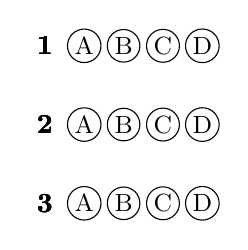
\begin{tikzpicture}[font=\small]
					\foreach \line in {1,2,3} {
						\begin{scope}[yshift=-\line cm]
							\foreach \letter/\position in {A/1, B/2, C/3, D/4} { 
								\node at (0,0) {\normalsize\textbf{\line}};
								\node[draw,circle,inner sep=1pt] at ({\position * 0.5},0) {\letter};
							}
						\end{scope}
					}
				\end{tikzpicture}\hspace{0.5in}
				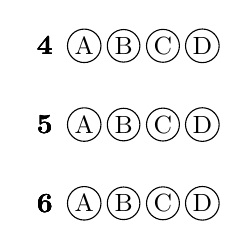
\begin{tikzpicture}[font=\small]
					\foreach \line in {4,5,6} {
						\begin{scope}[yshift=-\line cm]
							\foreach \letter/\position in {A/1, B/2, C/3, D/4} { 
								\node at (0,0) {\normalsize\textbf{\line}};
								\node[draw,circle,inner sep=1pt] at ({\position * 0.5},0) {\letter};
							}
						\end{scope}
					}
				\end{tikzpicture}\hspace{0.5in}	
				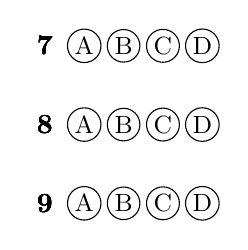
\begin{tikzpicture}[font=\small]
					\foreach \line in {7,8,9} {
						\begin{scope}[yshift=-\line cm]
							\foreach \letter/\position in {A/1, B/2, C/3, D/4} { 
								\node at (0,0) {\normalsize\textbf{\line}};
								\node[draw,circle,inner sep=1pt] at ({\position * 0.5},0) {\letter};
							}
						\end{scope}
					}
				\end{tikzpicture}\hspace{0.5in}
				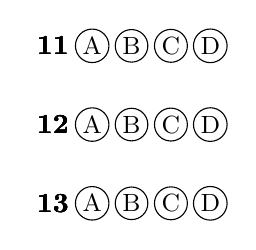
\begin{tikzpicture}[font=\small]
					\foreach \line in {11,12,13} {
						\begin{scope}[yshift=-\line cm]
							\foreach \letter/\position in {A/1, B/2, C/3, D/4} { 
								\node at (0,0) {\normalsize\textbf{\line}};
								\node[draw,circle,inner sep=1pt] at ({\position * 0.5},0) {\letter};
							}
						\end{scope}
					}
				\end{tikzpicture}\hspace{0.5in}
				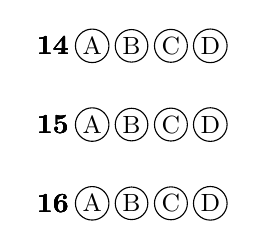
\begin{tikzpicture}[font=\small]
					\foreach \line in {14,15,16} {
						\begin{scope}[yshift=-\line cm]
							\foreach \letter/\position in {A/1, B/2, C/3, D/4} { 
								\node at (0,0) {\normalsize\textbf{\line}};
								\node[draw,circle,inner sep=1pt] at ({\position * 0.5},0) {\letter};
							}
						\end{scope}
					}
				\end{tikzpicture}	
			\end{document}